\documentclass[a4paper,10pt]{article}

% ============================================================
%                         Import Packages
% ============================================================
\usepackage[utf8]{inputenc}
\usepackage{multicol}
\usepackage{amsmath}
\usepackage{amssymb}
\usepackage{geometry}
\usepackage{titling}
\usepackage{setspace}
\usepackage{enumitem}
\usepackage{lipsum}
\usepackage{graphicx}
\geometry{margin=0.1in}

% ============================================================
%                     Title and Author Settings
% ============================================================
\setlength{\droptitle}{-5em}
\preauthor{\vspace{-2em} \begin{center} \setstretch{0.8}}
\postauthor{\end{center}}
\predate{\vspace{-2em} \begin{center} \setstretch{0.8}}
\postdate{\end{center}\vspace{-2em}}

\title{\setstretch{0.8}ECE121B Midterm Cheatsheet}
\author{\setstretch{0.8}Sonny Ding}
\date{\setstretch{0.8}\today}

\setlength{\columnsep}{0.5cm}

\begin{document}

\maketitle

% ============================================================
%                        Body Settings
% ============================================================
\raggedcolumns
\begin{multicols}{3}

\setstretch{0.8} % Adjust this value to make line spacing tighter

\setlength{\abovedisplayskip}{0pt}
\setlength{\belowdisplayskip}{0pt}

% ------------------------------------------------------------
%                      Crystal Structure
% ------------------------------------------------------------
\section*{Crystal structure}

Crystal is periodic. Unit cell may be:

\begin{itemize}[noitemsep, topsep=0pt, left=0pt]
    \item Simple cubic, $\frac{1}{8}\cdot 8 = 1$
    \item Body-centered cubic, $\frac{1}{8}\cdot 8 + 1 = 2$
    \item Face-centered cubic, $\frac{1}{8}\cdot 8 + \frac{1}{2}\cdot 6 = 4$
    \item Diamond / Zincblende, $\frac{1}{8}\cdot 8 + \frac{1}{2}\cdot 6 + 4 = 8$, like 2 FCCs shifted $(\frac{a}{4}, \frac{a}{4}, \frac{a}{4})$
\end{itemize}

Silicon is diamond, after calculation, $a = 5.43 \text{ \AA}$. Density is $5\times 10^{22} \text{ atoms/cm}^3$.

Miller indices: $(hkl)$ for plane, $[hkl]$ for direction. Plane is normal to direction.

% ------------------------------------------------------------
%                          Section 2
% ------------------------------------------------------------
\section*{Energy bands}

Classically, particles are $F=ma = m \frac{dv}{dt}$, waves are $\frac{\partial^2 u}{\partial t^2} = c^2 \left( \frac{\partial^2 u}{\partial x^2} + \frac{\partial^2 u}{\partial y^2} + \frac{\partial^2 u}{\partial z^2} \right)$.

But in quantum mechanics, waves are particle-like, as shown in de Broglie's relation $p = \frac{h}{\lambda} = \hbar k$.

Photoelectric effect: $E = hf$.

Uncertainty principle: $\Delta p \Delta x \ge \frac{\hslash}{2}, \Delta E \Delta t \ge \frac{\hslash}{2}$

Schrodinger equation: 

$\left(- \frac{\hslash^{2}}{2m}\nabla^{2}+U(r)\right)\psi = E\psi$

For different elements, their energy states are different, because they have different $U(r)$. Nature tends to want to go to a state that is stable with the minimum amount of energy, so given say a bunch of silicon, they will decrease their interatomic distance until it forms a valence band and a conduction band, with bandgap in between.

Brillouin zone is unit cell for reciprocal k space. K space is obtained using Fourier transform.

Classically, particles follow $E = \frac{p^2}{2m}$. Quantum mechanically, $E = \frac{\hbar^2 k^2}{2m}$. We may plot E vs k to get energy bands.

We make approximations to E-k diagrams at their minimum, as different parabolic equations:

\begin{align*}
    E &= \frac{\hslash^{2}k^{2}}{2m_{e}^{*}} \\
    \frac{d^{2}E}{dk^{2}} &= \frac{\hslash^{2}}{m_{e}^{*}} \\
    m_{e}^{*} &= \frac{\hslash^{2}}{\frac{d^{2}E}{dk^{2}}}
\end{align*}

Larger \textbf{effective mass} means slower electrons, flatter curve, smaller lattice constant. This makes sense since smaller lattice constant means tighter bonds, which means electrons are harder to move. That generally means larger bandgap too.

% ------------------------------------------------------------
%                          Section 3
% ------------------------------------------------------------
\section*{Density of states}

\textbf{Density of states} answers the question: how many states are there in a given energy range?

$$g(E) dE = \frac{m^* \sqrt{2 m^* E}}{\pi^2 \hslash^3} dE$$

If we change our points of reference energy level and effective mass, we obtain DOS for conduction band and valence band.

\begin{align*}
    g_c(E) &= \frac{\sqrt{2 m_n^{*3/2}} \, (E - E_C)^{1/2}}{\pi^2 \hbar^3} \\
    g_v(E) &= \frac{\sqrt{2 m_p^{*3/2}} \, (E_V - E)^{1/2}}{\pi^2 \hbar^3}
\end{align*}

\begin{center}
    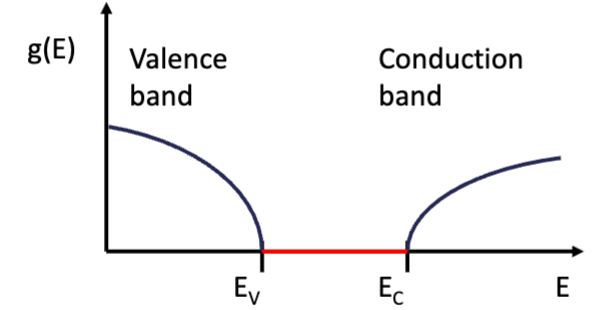
\includegraphics[width=\columnwidth]{../img/Pasted image 20241008113136.png}
\end{center}

\textbf{Fermi-Dirac distribution} answers the question: what is the probability of a state being occupied? There are other statistical distributions,

\begin{itemize}[noitemsep, topsep=0pt, left=0pt]
    \item Maxwell-Boltzmann distribution, for classical particles, particles distinguishable by number, with no limit on number of particles in each energy state
    \item Bose-Einstein distribution, for bosons, indisguinshable, no limit
    \item Fermi-Dirac distribution, for fermions, indisguinshable, with limit of 1 particle per state
\end{itemize}

$$f(E) = \frac{1}{1 + e^{\frac{E - E_F}{kT}}}$$

\begin{center}
    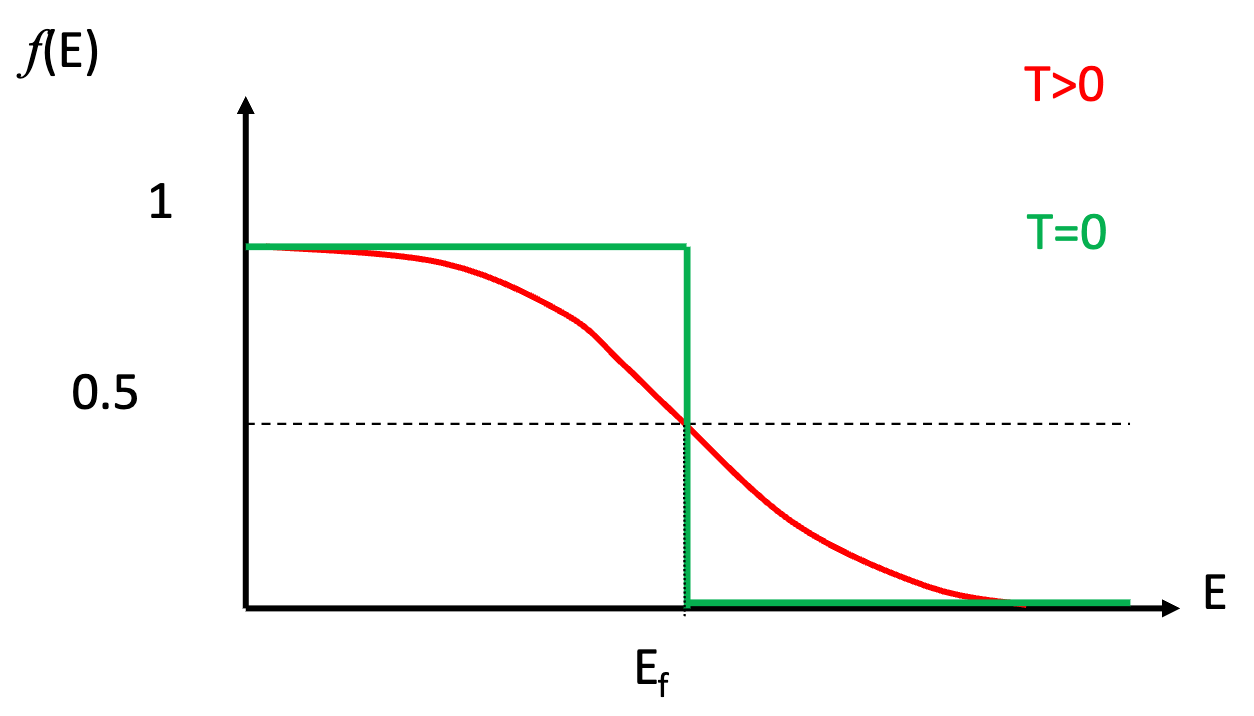
\includegraphics[width=\columnwidth]{../img/Pasted image 20241010102613.png}
\end{center}

In the middle is Fermi level. If $E-E_{F} >> 3k_{B}T$, we make the Boltzmann approximation by getting rid of the 1.

Concentration of carriers is obtained by multiplying density of states and Fermi-Dirac distribution. $n(E) = g_c(E)f(E), p(E) = g_v(E)[1-F(E)]$. Then, integrate each part to get total concentration of carriers.

\begin{align*}
    n &= 2 \left( \frac{m_n^* k_B T}{2\pi \hslash^2} \right)^{3/2} \exp \left( \frac{E_F - E_C}{k_B T} \right)\\
    p &= 2 \left( \frac{m_p^* k_B T}{2\pi \hslash^2} \right)^{3/2} \exp \left( \frac{E_V - E_F}{k_B T} \right)
\end{align*}

The non-exponential terms are known as $N_C, N_V$. Effective density of states.

For intrinsic materials, $n=p$. For extrinsic materials, $np = n_{i}^{2} = N_{C}N_{V}\exp(\frac{E_{C}-E_{V}}{k_{B}T})$.

For intrinsic materials, Fermi level is found by letting $n=p$, solve for $E_{F}$. The result is $E_i - E_V = \frac{E_c - E_V}{2} + \frac{3}{4} k_B T \ln \left( \frac{m_p^*}{m_n^*} \right)$, about at center between conduction and valence band.

\section*{Free carriers and dopants}

We can dope material to make its Fermi level move closer to conduction band or valence band. To make Fermi level closer to conduction band, dope shallow donors with donor states right below the conduction band, now the material is n-type. Deep donors are hole traps. A dopant is considered shallow if its binding energy is within $k_B T$.

A donor state is neutral when it is occupied, and is positively charged when it is empty. An acceptor state is neutral when it is empty, and is negatively charged when it is occupied.

\textbf{Fraction of dopant ionization} depends on temperature and binding energy.

$$\frac{1}{1+\frac{g_{D,A}N_{D,A}}{N_{C,V}}\exp(\frac{E_{B}}{k_{B}T})}$$

Due to different charge carrier concentration vs temperature, the device may be in freeze-out, intrinsic, or extrinsic region.

\begin{center}
    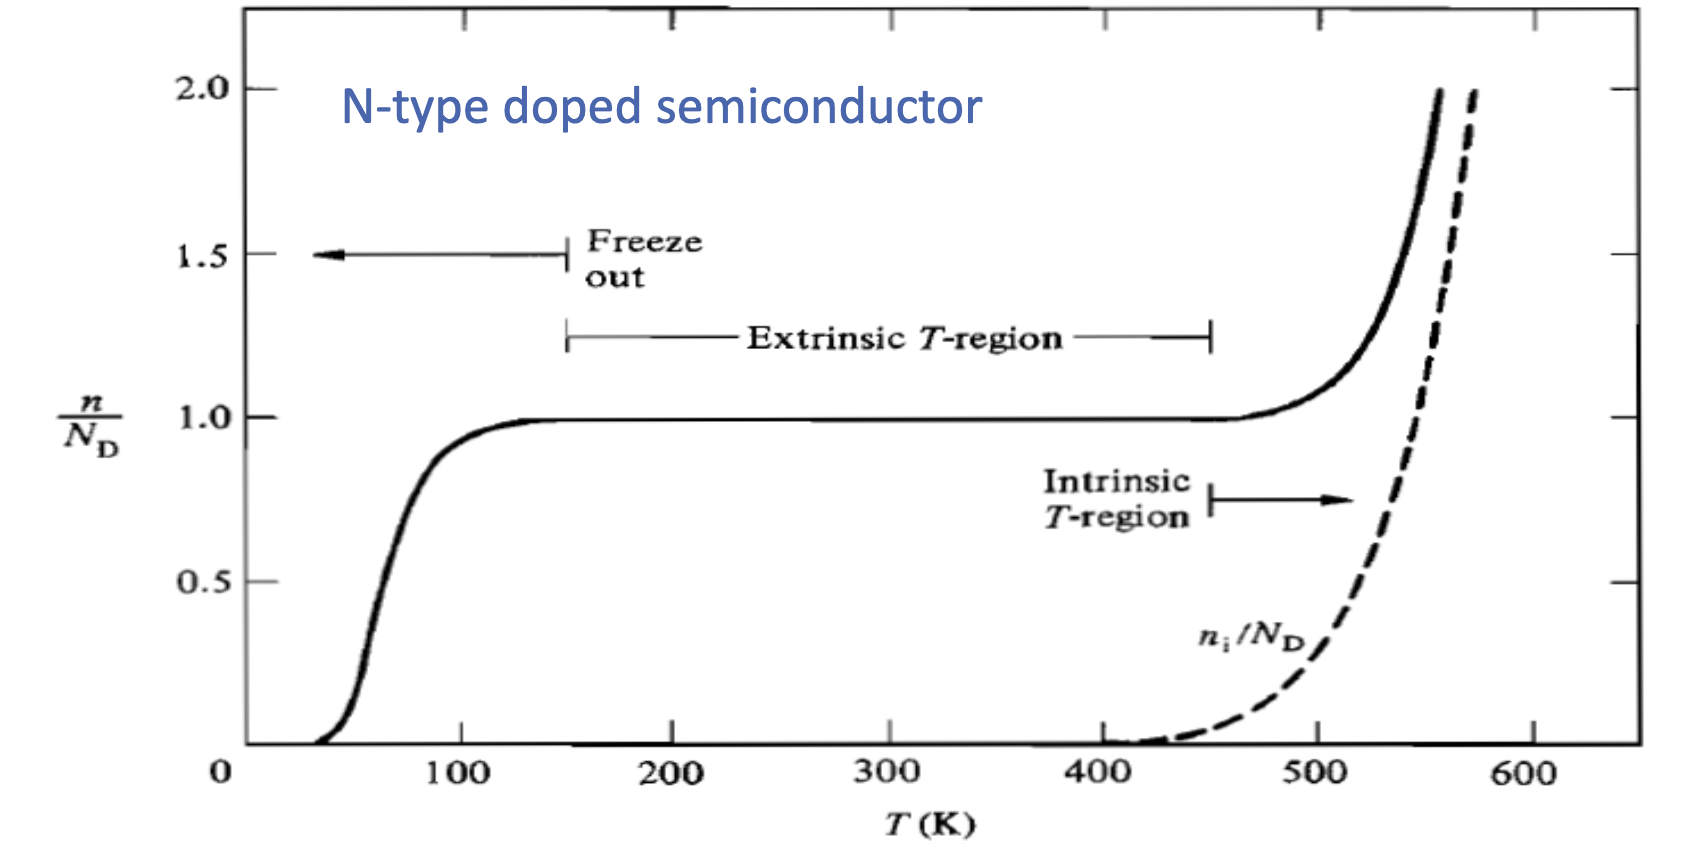
\includegraphics[width=\columnwidth]{../img/Pasted image 20241015105159.png}
\end{center}

Doping shifts Fermi level closer to them.

Remember Boltzmann approximation? If $E-E_{F} < 3k_{B}T$, the approximation will be broken.

\textbf{Doped carrier concentration} can be calculated by using charge neutrality: $q(p+N_{D}^{+}) = q(n+N_{A}^{-})$. 2 are mobile, 2 are fixed. Then, it should always be true that

\begin{small}
    \begin{align*}
        n &=  \frac{N_D - N_A}{2} + \sqrt{\left( \frac{N_D - N_A}{2} \right)^2 + n_i^2}\\
        p &=  \frac{n_i^2}{n} = \frac{N_A - N_D}{2} + \sqrt{\left( \frac{N_A - N_D}{2} \right)^2 + n_i^2}
    \end{align*}
\end{small}

Intrinsic just means $n=p=n_i$. Extrinsic means to pick the majority carrier concentration $N_A$ or $N_D$ and then $n_i^2/N$. If compensated, that is doping levels are approximate, then use the full equation.

At low temperatures, Fermi levels are primarily influenced by the doped materials and are closer to the valence or conduction band, and at high temperatures, silicon dominates so Fermi level moves back towards the intrinsic level.

\section*{Drift and diffusion}

There are fixed charges and free carriers, but only free carriers contribute to current.

\textbf{Drift current} is a result of electric field. $v_{avg} = \frac{q\tau}{m_{e}^{*}}\vec{E} = \mu \vec{E}$, $\mu$ is mobility. Note that since electrons and holes have different effective mass, their mobility and drift current is also different. Also, drift speed for electrons should change sign.

In reality, the drift current equation isn't quite accurate, as drift velocity saturates, and some materials do an "overshoot" since it gains so much energy so that it moves from one valley to another valley, and the effective mass changes.

Now, to study $\tau$, Mathieson's rule states $\frac{1}{\tau_{tot}} = \sum_{i} \frac{1}{\tau_{i}}$. Each $\tau$ is a scattering time resulted by a certain scattering mechanism, like by dopants, temperature, defects, alloy.

The dominating scattering mechanisms are:

\begin{itemize}[noitemsep, topsep=0pt, left=0pt]
    \item Phonon scattering, phonon is crystal vibration caused by temperature, so it dominates as temperature increases
    \item Ionized impurity scattering, at low temperature there is freeze-out, which means no carriers can form screening for the impurities, so it dominates at low temperature
\end{itemize}

\begin{center}
    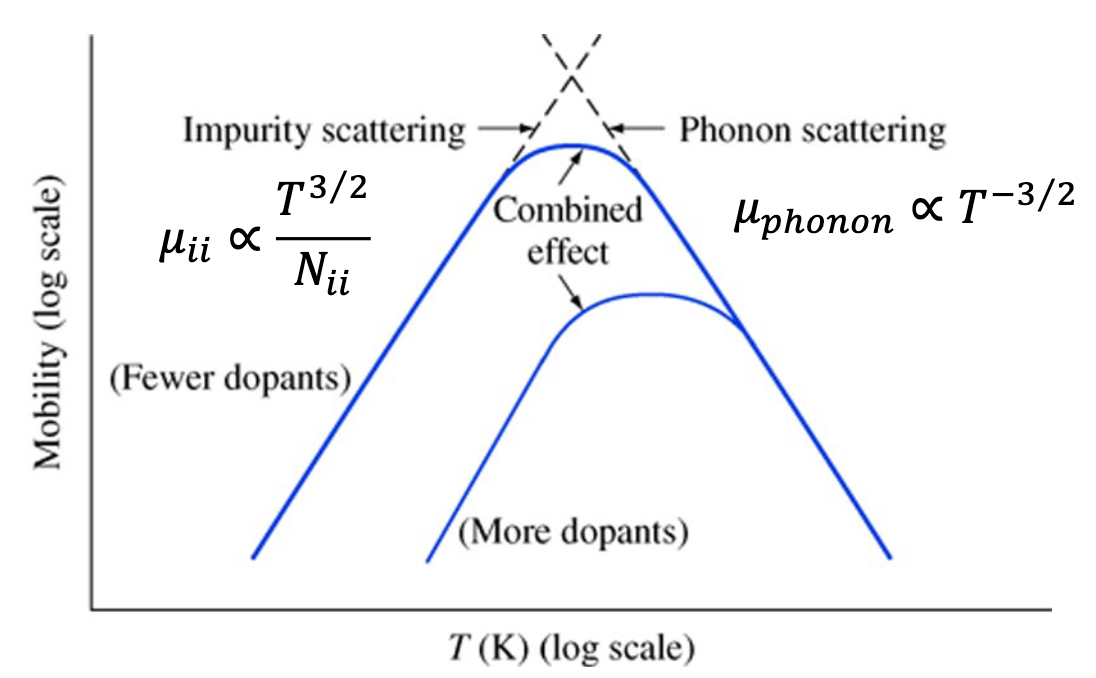
\includegraphics[width=\columnwidth]{../img/Pasted image 20241017111548.png}
\end{center}

\begin{align*}
    J_{p,drift} &= +qpv_{drift,p} &&= +qp\mu_{p}\mathcal{E}\\
    J_{n,drift} &= -qnv_{drift,n} &&= +qn\mu_{n}\mathcal{E}
\end{align*}

Electron drift velocity is negative, but since its charge is also negative, both drift currents are in the same direction. So conductivity is $\sigma = \rho^{-1} = q(n\mu_{n}+p\mu_{p})$. $\rho$ is resistivity.

\textbf{Diffusion current} is a result of concentration gradient. $J_{n,diff} = -qD_{n}\frac{dn}{dx}$, $J_{p,diff} = +qD_{p}\frac{dp}{dx}$. $D_n, D_p$ are diffusion coefficients.

\begin{align*}
    J_{n}&=  + q\mu_{n}n\vec{E} + qD_{n} \frac{dn}{dx}\\
    J_{p}&=  + q\mu_{p}p\vec{E} - qD_{p} \frac{dp}{dx}
\end{align*}

\textbf{Equilibrium condition} is defined as no external stimuli \textit{and} no net current flow. So, a piece of semiconductor can have no net current when light shines on it, but it is only in steady state, not in equilibrium.

By definition, $E_F$ is constant if it is in equilibrium. 

$E = -qV, \mathcal{E} = -\nabla V = \frac{1}{q} \frac{dE_{C}(x)}{dx}$.

\begin{center}
    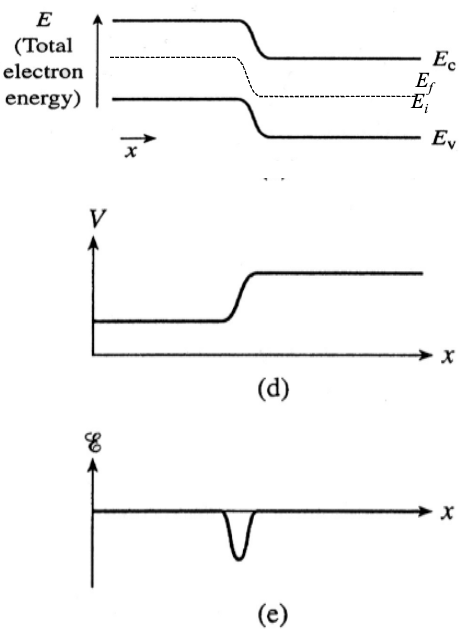
\includegraphics[width=0.5\columnwidth]{../img/Pasted image 20241022104107.png}
\end{center}

Under equilibrium, following equations hold:

\begin{align*}
    J_{total,n} &= +qn\mu_{n}\mathcal{E} + qD_{n}\frac{dn}{dx} = 0\\
    n(x) &= n_{i}\exp{\left(\frac{E_{F}(x)-E_i(x)}{k_{B}T}\right)}
\end{align*}

Solve these equations we have 2 observations. 1. $\frac{dE_F}{dx}=0$. 2. $\frac{D_{n}}{\mu_{n}} = \frac{k_{B}T}{q}, \frac{D_{p}}{\mu_{p}} = \frac{k_{B}T}{q}$. Second term is Einstein relationship.

\section*{Generation recombination}

Generation and recombination describe the process of creating and destroying carriers. They tend to restore equilibrium.

\begin{itemize}[noitemsep, topsep=0pt, left=0pt]
    \item Band to band, may be thermal or optical
    \item At R-G center, also known as Shockley-Read-Hall recombination, indirect recombination
    \item Auger recombination and impact ionization, send energy to lattice to other carriers, may cause avalanche if field of impact ionization is high
\end{itemize}

To describe R-G quantitatively, assess majority/minority carrier. $n_0, p_0$ are equilibrium carrier concentration. $n, p$ are non-equilibrium carrier concentration. $G, R$ are generation and recombination rate.

When not under equilibrium, $n_i^2 \ne np$. But $n_i^2 = n_0 p_0$ is always true.

Low level injection means R-G affects minority carriers strongly but not majority carriers.

So, assume low level injection, equaiton for R-G center recombination rate is $\frac{dp}{dt}|_{R} = -c_{p}N_{T}p$. $c_p$ is capture coefficient of holes, $N_T$ is R-G center concentration. If under equilibrium, $\frac{dp}{dt}|_{G_{eq}} = \frac{dp}{dt}|_{G} = c_{p}N_{T}p_{0}$ to cancel out. We can also just approximate its non-equilibrium as equilibrium. In total, $\left.\frac{dp}{dt}\right|_{i-\text{thermal},R-G} = \left.\frac{dp}{dt}\right|_{R} + \left.\frac{dp}{dt}\right|_{G} = -c_{p}N_{T}(p - p_{0}) = -c_{p}N_{T}\Delta p = -\frac{\Delta p}{\tau_p}$. $\tau$ is minority carrier lifetime.

Photogeneration rate is $G_{L}(x,\lambda) = G_{L0}e^{-\alpha x}$ as current is $I = I_{0}e^{-\alpha (\lambda)x}$.

Direct bandgap materials like GaAs are good for optical generation, since it requires only $\Delta E$ or photons and almost no $\Delta k$ or photons. Indirect bandgap materials like Si are bad for optical generation, since it requires both $\Delta E$ and $\Delta k$.

\section*{Current continuity}

$\frac{\partial n}{\partial t} A\,dx = \left[\frac{J_{n}(x)A}{-q}-\frac{J_{n}(x+dx)A}{-q}\right] + (G-R)A\,dx$. Left side checks change in carrier density over distance. Right square bracket represents the net current density flow in and out, a consequence of carrier movement. Last term is G-R, which controls number of carriers.

$\frac{\partial n}{\partial t} = \frac{1}{q} \nabla\cdot\vec{J_{n}} + \left.\frac{\partial n}{\partial t}\right|_{thermal R-G} + \left.\frac{\partial n}{\partial t}\right|_{other R-G}$ is the formal continuity equation. Add negative size for J term for holes.

We may make assumptions to simplify the equation.

\begin{itemize}[noitemsep, topsep=0pt, left=0pt]
    \item 1 dimension
    \item Only consider minority carriers
    \item $\vec{E} = 0$, so ignore drift
    \item Carrier concentration is not a function of position
    \item Assume low level injection
    \item Assume R-G center as main R-G
    \item Assume only other R-G is optical
\end{itemize}

After simplification we get

$$\frac{\partial \Delta n_p}{\partial t} = D_n \frac{\partial^2 \Delta n_p}{\partial x^2} - \frac{\Delta n_p}{\tau_n} + G_L$$

No signs change for electrons. Further simplify depends on situation: $\frac{\partial \Delta n}{\partial t} \rightarrow 0$ if steady state, other terms may also be 0 if say there is no minority carrier gradient, or no thermal R-G or no light.

\textbf{Maybe write the common solutions?}

\end{multicols}

\end{document}


